\documentclass{xduugthesis}
\usepackage{amsmath}
\usepackage{amssymb} 
\usepackage{graphicx}
\usepackage{epstopdf}

\xdusetup{
 style = { cjk-font = win, latin-font = tac },
 info = {
abstract = {text/abstract_en.tex},
abstract* = {text/abstract_ch.tex},
keywords = {三维重建,点云数据,神经符号距离函数,神经网络},
 keywords* = {3D Reconstruction,Point Cloud Data,Neural Signed Distance Function,Neural Network}
 }
 }

\begin{document}

\chapter{绪论}
\section{研究背景}
三维重建技术作为计算机视觉与三维建模领域的关键研究方向，近年来受到了学术界与工业界的广泛关注。点云数据作为三维重建技术的核心基础，正逐渐成为该领域研究的热点。点云数据的获取方式多样，既可以借助先进的三维扫描设备（如激光雷达）直接获取，也可以通过基于多视图几何的图像处理方法间接提取。这些方法所获取的点云数据能够以极高的精度和分辨率，精准地呈现物体或场景的三维几何特征，为后续的三维重建工作提供了丰富的细节信息。

随着传感器技术的不断发展，激光雷达等三维扫描设备的性能日益提升，其扫描精度、分辨率和数据采集速度都得到了显著提高。同时，计算能力的飞速发展也为点云数据的处理和分析提供了强大的支持。高性能计算机和图形处理单元（GPU）的广泛应用，使得复杂的点云数据处理算法能够在短时间内完成计算任务，从而大大提高了点云数据的处理效率。这些技术进步使得点云数据的获取过程愈发便捷高效，为三维重建技术的进一步发展奠定了坚实的数据基础，推动了该技术在多个领域的广泛应用。

在众多实际应用场景中，点云三维重建技术的应用价值愈发凸显。在自动驾驶领域，激光雷达所获取的点云数据是实现车辆环境感知与障碍物检测的关键。通过点云数据，车辆能够实时感知周围三维空间环境，准确识别道路、建筑物、行人以及其他车辆等物体的位置和形状，从而为自动驾驶系统的决策提供重要依据。在文化遗产保护领域，点云技术被广泛应用于文物的高精度三维重建。通过对文物进行三维扫描，获取其表面的点云数据，再利用先进的三维重建算法，可以构建出文物的高精度三维模型。这些三维模型不仅能够为文物的保存和修复提供精确的参考，还可以通过数字化手段进行展示和传播，让更多人能够欣赏和了解文化遗产。

在电磁仿真领域。传统电磁仿真技术因依赖人工构建三角网格模型，难以满足信道仿真、车载毫米波雷达及SAR成像等领域对真实场景1:1还原的迫切需求。激光雷达点云重建技术凭借其低成本、高效率的三维数据采集能力，正在重塑这一技术格局——通过亚厘米级精度的现实表征，点云重建数据不仅解决了电磁仿真中目标建模的瓶颈，更为多领域数字化转型提供了全新解决方案。

此外，点云三维重建技术在工业设计、虚拟现实、游戏开发等多个领域也展现出巨大的应用潜力。在工业设计中，点云数据可用于快速构建产品的三维模型，为产品设计和优化提供直观的参考；在虚拟现实和游戏开发中，点云重建的三维场景能够为用户带来更加逼真的沉浸式体验。因此，点云三维重建技术正逐渐成为推动相关领域发展的重要技术手段，其应用前景广阔，具有重要的现实意义。

在众多实际应用场景中，点云三维重建技术的应用价值愈发凸显。在自动驾驶领域，激光雷达所获取的点云数据是实现车辆环境感知与障碍物检测的关键。通过点云数据，车辆能够实时感知周围三维空间环境，准确识别道路、建筑物、行人以及其他车辆等物体的位置和形状，从而为自动驾驶系统的决策提供重要依据。在文化遗产保护领域，点云技术被广泛应用于文物的高精度三维重建。通过对文物进行三维扫描，获取其表面的点云数据，再利用先进的三维重建算法，可以构建出文物的高精度三维模型。这些三维模型不仅能够为文物的保存和修复提供精确的参考，还可以通过数字化手段进行展示和传播，让更多人能够欣赏和了解文化遗产。此外，点云三维重建技术在工业设计、虚拟现实、游戏开发等多个领域也展现出巨大的应用潜力。在工业设计中，点云数据可用于快速构建产品的三维模型，为产品设计和优化提供直观的参考；在虚拟现实和游戏开发中，点云重建的三维场景能够为用户带来更加逼真的沉浸式体验。因此，点云三维重建技术正逐渐成为推动相关领域发展的重要技术手段，其应用前景广阔，具有重要的现实意义。
\section{国内外研究现状}
激光雷达技术作为一种主动遥感技术，因其获取点云高精度和高分辨率的特点，在3D数据获取中扮演着重要角色。然而，三维点云通常不足以建模复杂物理结构。相比点云的离散化表面表示，在实际应用中需要物体或场景的连续表面表示。因此，将点云转换为可以更灵活地表示某些几何形状的mesh网格(称为表面重建)，是数字几何处理中的一个核心问题。雷达点云重建是指从雷达系统捕获的点云数据中恢复出物体表面的三维形状，这一技术在自动驾驶、城市规划、环境监测等多个领域有着广泛的应用。

传统点云重建方法主要依赖于几何算法，如1983年Edelsbrunner et al.提出的alpha shapes算法，是对凸包的推广，获得的三角网格是Delaunay三角网格的子集。1999 Bernardini et al.提出Ball pivoting算法，它和alpha shapes相关，但是更简单鲁棒高效，通过选择种子三角形并沿边轴旋转去拓展网格边界的方法来获取mesh重建结果。相比于前面显式网格重建算法，Kazhdan et al.在2006提出一种隐式表面重建算法：Poisson表面重建。在空间中引入指数函数，构建平滑指示函数的梯度和物体表面法向量场的关系。并巧妙转换为Poisson方程，采用求解线性方程组的方式去求解Poisson方程解，最后利用marching cubes提取物体等值面，得到相比于上述重建算法更为平滑的重建曲面。尽管这些传统点云重建方法可以有效重建曲面。但这些方法在处理噪声、缺失数据和异常值方面存在局限性，特别是针对非均匀采样和点云稀疏场景，效果会大打折扣。 

近年来，随着深度学习技术发展，基于深度学习的点云重建方法取得显著进展。这些方法能够从数据中直接学习输入点云和期望表面的性质，减少了手动参数调整的需求。例如从表面插值入手，Sharp et al.在2020年提出一种从初始候选三角形集合中迭代构造三角划分的PointTriNet方法,其中第一个网络基于概率选择种子三角形，接着第二个网络由被选择三角形的相邻点形成新三角形。接着，新的三角形再被第一个网络处理。在表面拟合方面，2018年由Groueix et al.提出AtlasNet，在曲面重建领域开创性采用基于深度学习的方法，从三角化2D面片开始，使用神经网络来调整其顶点位置。通过最小化形变表面和点云之间距离来训练网络。在基于体积插值的重建算法中，2021年Luo et al.提出DeepDT网络，使用在三维Delaunay化中操作的图神经网络去预测全局能量参数。在基于体积拟合的重建算法中，Huang et al.在2023年提出神经核表面重建NKSR技术，将学习到的特征与经典泊松表面重建技术相结合，用一种名为神经核场的新型3D深度学习方法来实现高质量的重建。由此可见，深度学习方法在点云重建领域的应用正变得越来越广泛。这些方法能够处理更复杂的形状类别，并在面对真实世界数据中的各种异常时表现出更好的鲁棒性。

点云重建技术正迅速发展，深度学习方法的引入为这一领域带来了新的机遇。随着技术的进步和应用需求的增长，预计未来将有更多的创新方法被提出，以解决现有挑战并推动该领域的进一步发展。这些创新方法可能会包括更高效的数据处理技术、更精确的模型训练策略以及更强大的硬件支持，从而使得点云重建技术在各个行业中得到更广泛的应用。

\section{本文研究目标与内容}

本文旨在探索激光雷达点云数据的高精度三维重建技术，通过对比传统算法与新兴的基于深度学习的隐式重建方法，分析其性能差异，并验证其在实际应用中的表现。具体研究目标为首先深入研究传统显示三维表面重建算法（如Alpha Shapes和Ball Pivoting Algorithm）和基于深度学习的隐式重建方法（如StEik），分析其理论基础、算法框架及其在点云数据处理中的性能差异。其次是，从开源三维点云数据集和自采集数据集中验证不同算法的性能。 

全文共分为五章，内容如下：

第一章是绪论，首先，对三维重建，激光雷达点云等研究意义作了简明的介绍。之后，说明了激光雷达点云三维重建的研究意义，国内外的研究现状和目前进行的主要研究趋势，为后续章节铺垫了基础。

第二章是传统三维表面重建研究，详细介绍传统三维表面重建算法的基本理论和算法框架，包括Alpha Shapes和Ball Pivoting Algorithm（BPA）滚球算法。

分析这些传统算法在点云数据处理中的优势和局限性。

第三章是基于神经网络的三维表面重建研究，深入研究基于神经符号距离函数的隐式重建方法StEik， 分析StEik算法在处理复杂点云数据时的性能表现。

第四章是三维表面重建算法的仿真验证，利用3D打印技术和三维扫描仪采集精确点云数据集，构建自采集数据集。对比不同算法在自采集数据集上的性能，验证不同算法在复杂场景中的实际应用能力。通过实验结果，分析算法在实际工程应用中的稳定性和适应性，为技术方案的提出提供实验依据。

第五章是总结与展望，总结本文的研究成果，解析研究过程中存在的问题和不足，对未来的研究方向进行展望，提出进一步改进和优化的建议。

\chapter{传统三维表面重建研究}
\section{Alpha Shapes重建算法}
\subsection{算法介绍}
Alpha Shapes是一种用于从点集构造形状的几何算法，由Edelsbrunner等人提出。它在计算几何、计算机图形学、地理信息系统等领域有着广泛的应用，特别是在曲面重建、形状分析和数据可视化等方面。它通过参数化的方式描述点集的形状，能够捕捉从局部细节到整体结构的几何特征。Alpha Shapes的核心思想是利用一个参数$\alpha$控制形状的细节程度，通过调整$\alpha$的值，可以生成一系列从精细到粗略的形状表示。二维的Alpha Shapes如图 \ref{fig2.1} 所示。
\begin{figure}[htbp]
\centering
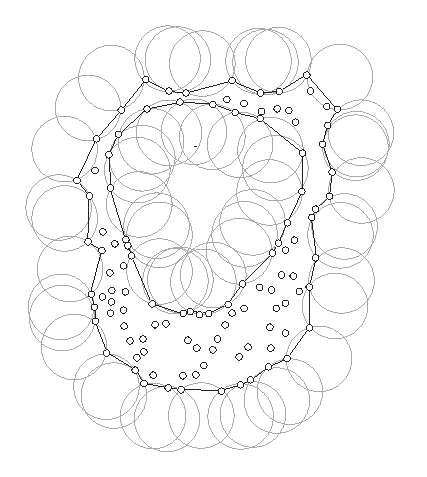
\includegraphics[scale=1]{2.1.eps}
\caption{二维Alpha Shapes效果}
\label{fig2.1}
\end{figure}
给定一个点集 \( S \subset \mathbb{R}^d \)（\( d \) 通常为 2 或 3），Alpha Shapes 是一个与参数 \( \alpha \) 相关的几何形状。直观上，可以想象用一个半径为 \( \alpha \) 的球体（在二维中是一个圆）在这个空间中移动，雕刻出所有球体能够触及的区域。所能触及的区域的边界即为 Alpha Shapes，直观地描述揭示了 Alpha Shapes 的基本思想：通过调整球体的半径 \( \alpha \)，可以捕捉到点集的不同层次的形状特征。当 \( \alpha \) 趋近于 0 时，Alpha Shapes 退化为点集本身；当 \( \alpha \) 趋近于无穷大时，Alpha Shapes 趋近于点集的凸包。通过调整 \( \alpha \) 的值，可以在不同层次上捕捉点云的几何结构。

Alpha Shapes 的定义基于点集的 Delaunay 三角剖分。Delaunay 三角剖分是一种将点集划分为非重叠的三角形或四面体的几何结构，其特点是每个三角形的外接圆或外接球不包含点集中的其他点。这种独特的性质确保了三角剖分的局部最优性，即每个三角形的内角尽可能接近 60 度，从而避免了出现过尖或过扁的三角形。Alpha Shapes 通过引入一个参数 \( \alpha \)，进一步扩展了 Delaunay 三角剖分的概念，允许在点集中识别出空洞和复杂的边界结构。当 \( \alpha \) 值较大时，Alpha Shapes 趋向于产生较为平滑的形状，而当 \( \alpha \) 值较小时，它能够保留更多的细节，包括点集中的空洞。
\subsection{算法基本原理}
Alpha Shapes的边界是由一系列满足特定条件的几何元素构成的，这些元素被称为“单纯形”（simplex）。simplex是几何学中的一个基本概念，它是三角形和四面体在任意维度上的推广。例如，在一维空间中，simplex是一个线段；在二维空间中，它是一个三角形；而在三维空间中，simplex则是一个四面体。

假设点集 \( S \) 中的点处于一般位置，在此背景下，一般位置的含义是：\( S \) 中没有 4 个点共面，也没有 5 个点共球；此外，还假设，对于任意固定的半径 \( \alpha \)，通过 \( S \) 中任意 2 个、3 个或 4 个点最小球的半径与 \( \alpha \) 不同。这种假设保证了对于每一个 \( T \subset S \)，当 \( |T| = k + 1 \leq d \) 时，多面体 \( \Delta T = \text{conv} \, T \) 恰好具有 \( k \) 维，因此是一个 \( k \)-simplex \( \Delta T \)。

Alpha Shapes 的边界由一系列满足特定条件的 \( \Delta T \) 构成，这些 \( \Delta T \) 被称为 \( \alpha \)-暴露（\( \alpha \)-exposed）。具体来说，一个单纯形被称为 \( \alpha \)-exposed，当且仅当存在一个半径为 \( \alpha \) 的空球，这个空球不包含点集中的任何其他点，并且该 simplex 恰好位于这个空球的边界上。数学表达为：对于 \( 0 \leq \alpha \leq \infty \)，定义一个 \( \alpha \)-球为半径为 \( \alpha \) 的开球。此外，\( \alpha \) 为0的球视为一个点，而 \( \alpha \) 为无穷的球视为一个开半空间。如果某个位于特定位置的 \( \alpha \) 球 \( b \) 与点集 \( S \) 的交集为空（即 \( b \cap S = \emptyset \)），则称这个 \( \alpha \) 球 \( b \) 是空的。基于此定义，若存在一个空的 \( \alpha \) 球，使得 \( T \) 中的点恰好是该球边界（当 \( d=3 \) 时为球面，当 \( d=2 \) 时为圆）与点集 \( S \) 的交集（即 \( T = \partial b \cap S \)），则称 \( k \)-simplex \( \Delta T \) 是 \( \alpha \)-exposed 的。二维\( \alpha \)-暴露如下图 \ref{fig2.2} 所示。
\begin{figure}[htbp]
\centering
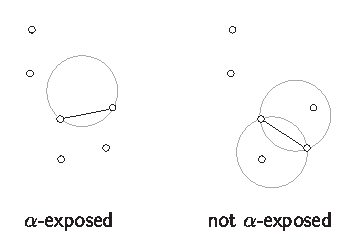
\includegraphics[scale=1.2]{2.2.eps}
\caption{\( \alpha \)-暴露示意图}
\label{fig2.2}
\end{figure}
\( \alpha \)-exposed 的 \( k \)-simplex \( \Delta T \) 是 Alpha Shapes 算法中用于确定形状边界的关键概念。它通过存在一个空的 \( \alpha \) 球且球的边界与 \( \Delta T \) 的顶点相交来定义。\( \Delta T \) 与 Delaunay 三角剖分有密切的关系。具体来说，如果一个 \( \Delta T \) 是 \( \alpha \)-exposed 的，那么它必定属于 Delaunay 三角剖分 \( DT(S) \)。这是因为 Delaunay 三角剖分中的 \( \Delta T \) 满足空外接球的条件，而 \( \alpha \)-exposed 的 \( \Delta T \) 的定义也涉及空球的条件。也就是说 Alpha Shapes 得到的是 Delaunay 三角剖分的一个子集，这也为得到点集 Alpha Shapes 提供了快速的方法。可以先生成点集的 Delaunay 三角剖分，接着在这个集合里面根据 \( \alpha \) 参数筛选出真正的 Alpha Shapes 三角 mesh。

Alpha Shapes 的计算依赖于 AlphaComplex \( C_\alpha(S) \)。\( C_\alpha(S) \) 是由所有满足 \( \alpha \)-exposed 条件的 \( \Delta T \) 组成的集合。它是 Delaunay 三角剖分的一个子复形，用于高效地表示点集的几何结构。具体来说：\( C_\alpha(S) \)通过筛选 Delaunay 三角剖分中的 simplex，保留那些满足 \( \alpha \)-exposed 条件的 \( \Delta T \)，从而构建出点集的几何形状。并且 \( C_\alpha(S) \) 的几何实现可以通过取凸包来完成，这使得它在计算上更加高效。

对于给定的点集 \( S \subset \mathbb{R}^d \) 和 \( 0 \leq \alpha \leq \infty \) 点集 \( S \) 关于 \( \alpha \) 的 \( C_\alpha(S) \) 包含所有满足以下条件的 \( \Delta T \in DT(S) \)：

第一，\( \Delta T \) 的外接圆或外接球半径小于 \( \alpha \)，且该球为空，或者

第二，\( \Delta T \) 是其他属于 \( C_\alpha(S) \) 的 simplex 的一个面。

AlphaComplex 的边界即为 Alpha Shapes 的边界。通过遍历 Delaunay 三角剖分中的所有 simplex，并应用上述条件，可以高效地计算出 Alpha Shapes。
\subsection{实现步骤}
Alpha Shapes算法的实现步骤如下：

第一，构建 Delaunay 三角剖分；对输入的点集 \( S \) 进行 Delaunay 三角剖分得到 \( DT(S) \)。

第二，对于所有属于 \( DT(S) \) 的 \( \Delta T \) 进行检验是否为 \( C_\alpha(S) \)。如果 \( \Delta T \) 的外接圆或外接球半径小于 \( \alpha \)，且该球为空。那么接受 \( \Delta T \) 连带着构成 \( \Delta T \) 的所有面作为 \( C_\alpha(S) \)。

第三，提取边界；所有 \( d \) 维的 \( C_\alpha(S) \) 构成了 Alpha Shapes \( S_\alpha \) 的内部，所有在边界 \( \partial C_\alpha(S) \) 构成了 \( \partial S_\alpha \) 的边界。

其中第二部分的算法具体来说是，对于每个 \( d \) 维 \( \Delta T \in DT(S) \)，计算每个 \( \Delta T \) 的外接球半径 \( \sigma_T \)。得到每个 \( d \) 维的 \( \Delta T \) 的区间 \( I_T = (\sigma_T, \infty) \)。接下来，对每个 \( k < d \) 维度的 \( \Delta T \in DT(S) \) 计算低纬度的区间 \( (a, b) \)。对于每个低维单纯形 \( \Delta T \)，需要根据其“超单纯形”（即包含 \( \Delta T \) 的更高维度单纯形）的区间来确定其属于 \( \alpha \)-complex 的条件。\(a, b\)为
\begin{equation}
a = \min \{a_U \mid B_U = (a_U, b_U), \Delta_U \text{ (k + 1)-Simplex}, T \subset U, U \subset C_\alpha\}
\end{equation}
\begin{equation}
b = \max \{a_U \mid B_U = (a_U, b_U), \Delta_U \text{ (d)-Simplex}, T \subset U, U \subset C_\alpha\}
\end{equation}

这样就可以根据 \(a, b, I_T\) 和 \(\alpha\) 的关系进行判断
\begin{equation}
\begin{cases}
\alpha \in I_T, & \text{则} \Delta T \text{属于} C_\alpha \\
\alpha \in (a, b), & \text{则} \Delta T \text{属于边界} \partial S_\alpha \\
\alpha \in (b, \infty), & \text{则} \Delta T \text{属于内部} \text{int}(S_\alpha)
\end{cases}
\end{equation}
三维Alpha Shapes结果如下图\ref{fig2.3}所示。其中从左到右子图的\(\alpha\)逐渐增大。
\begin{figure}[htbp]
\centering
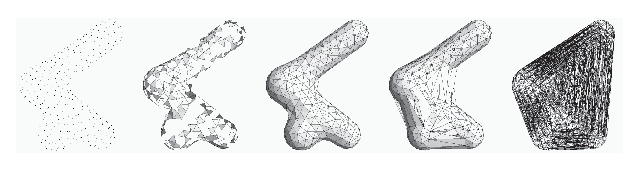
\includegraphics[scale=1.4]{2.3.eps}
\caption{三维Alpha Shapes效果}
\label{fig2.3}
\end{figure}
这种算法的优点是通过一次计算 Delaunay 三角剖分，可以得到所有可能的 \(\alpha\)-shape，而不需要对每个 \(\alpha\) 值重新计算。算法输出的是一个区间表示，可以根据不同的 \(\alpha\) 值快速得到对应的 \(\alpha\)-shape。并且基于 \(\alpha\)-complex 的定义和性质，算法的正确性得到了理论保证。

尽管 Alpha Shapes 在形状重建中具有广泛的应用，但也存在一些局限性。首先，参数 \(\alpha\) 的选择具有一定的主观性，通常需要通过试错法确定。其次，对于非均匀采样的点云，Alpha Shapes 可能无法准确重建目标形状。此外，传统的 Alpha Shapes 对于复杂形状的细节捕捉能力有限，尤其是在处理具有细长结构或高密度点云时。当\(\alpha\)过大时候，则会导致细节部分的丢失，如下图\ref{fig2.4}所示。左子图的\(\alpha\)合适，而右子图的\(\alpha\)过大。
\begin{figure}[htbp]
\centering
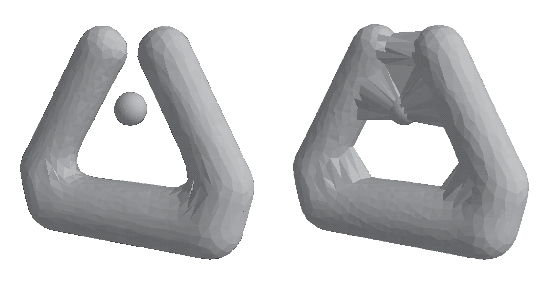
\includegraphics[scale=1]{2.4.eps}
\caption{ \(\alpha\)缺点示意图}
\label{fig2.4}
\end{figure}
为了克服这些局限性，后续研究提出了一些改进方法，例如加权Alpha Shapes和各向异性Alpha Shapes。这些方法通过引入权重或调整球的形状，提高了对复杂点云的适应性。
\section{BPA算法}
\subsection{算法介绍}
BPA算法是一种用于从三维点云数据中重建表面的高效方法，由Bernardini等人在1999年提出。该算法的核心思想是通过一个球体在三角形边缘周围旋转，当球体接触到三个点且不包含其他点时，就添加一个新的三角形。BPA算法与AlphaShapes理论密切相关，通过球体的旋转来构建三角形，从而形成一个表面重建。该算法特别适用于从密集的点云数据中重建表面，因为其效率和简单性使其成为一种流行的选择。BPA算法的二维示意图如下图\ref{fig2.5}所示。
\begin{figure}[htbp]
\centering
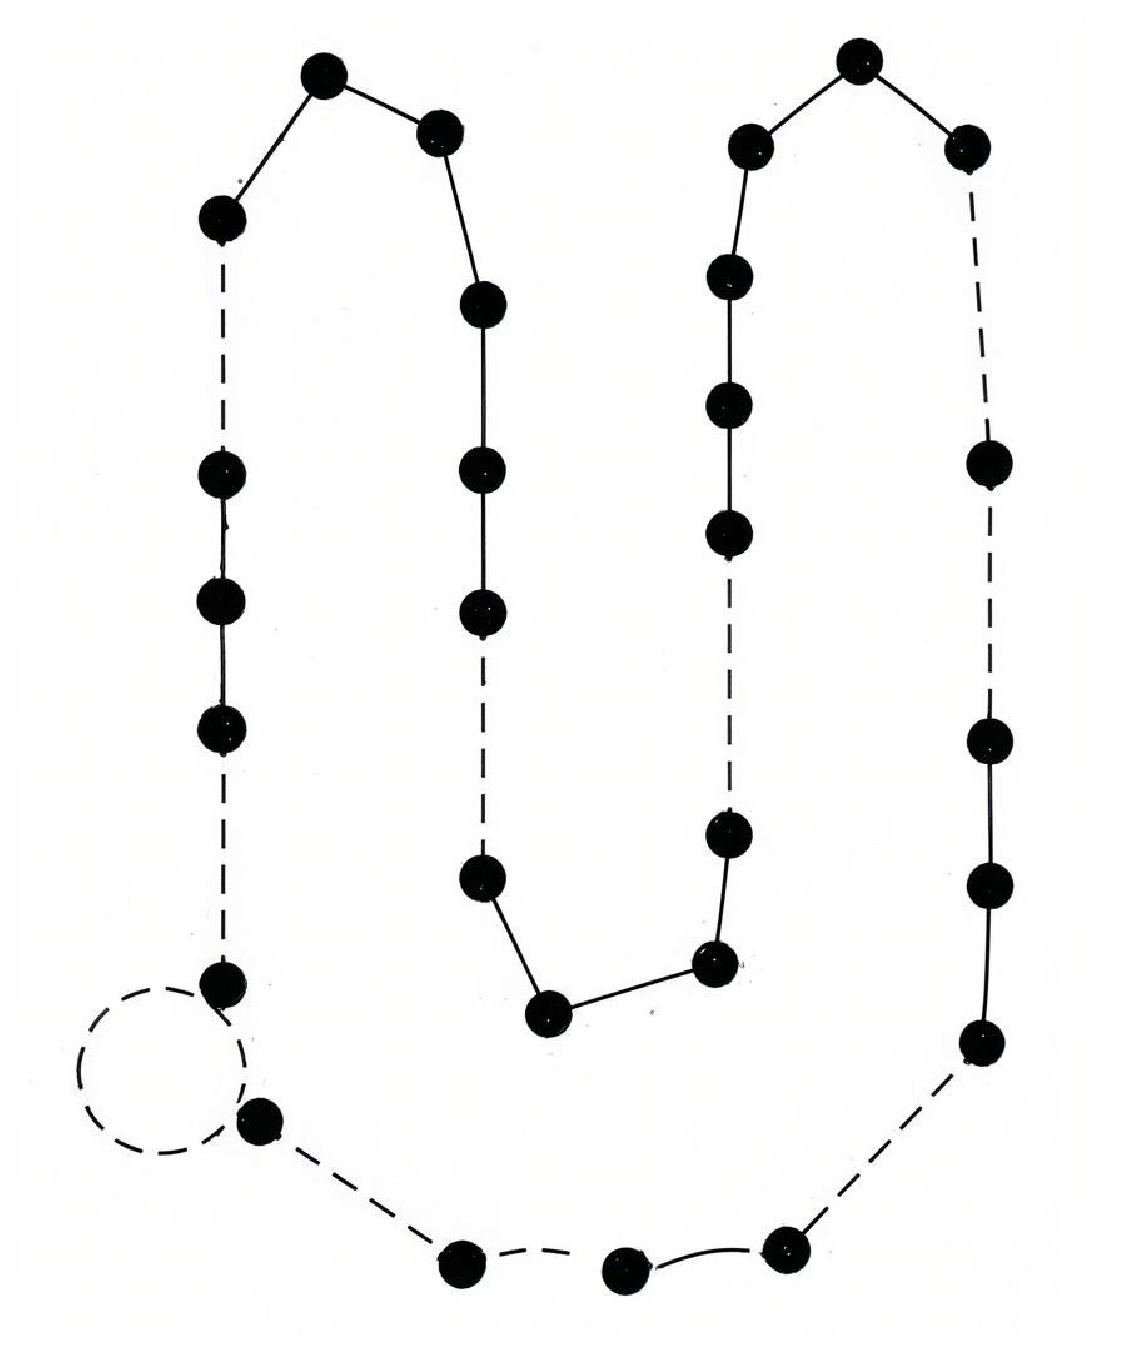
\includegraphics[scale=0.5]{2.5.eps}
\caption{BPA二维示意图}
\label{fig2.5}
\end{figure}

在实现过程中，BPA算法首先需要寻找一个种子三角形。这个步骤是通过在点云中搜索满足条件的三个点来完成的。一旦找到种子三角形，算法通过围绕边缘旋转半径为r的球体来添加新的三角形。这个过程会不断扩展三角形的前沿，直到没有更多的前沿边缘。为了确保重建的表面与输入点的法线方向一致，算法在创建每个三角形时都会检查其法线方向是否与顶点法线方向一致。此外，BPA算法还包含一个后处理步骤，用于填充由于数据缺失或法线方向错误导致的孔洞。

BPA算法的实现依赖于两个重要的数据结构：搜索结构和表面网格结构。搜索结构通常使用八叉树来快速访问给定位置的范围邻域。八叉树将空间划分为包含点的单元格，加速了邻域查询。表面网格结构则描述了一个带有边界的流形，包括三角形面片、边和顶点。每个顶点存储其相邻的三角形和边，每条边存储其两个端点和最多两个相邻的面片。这种数据结构确保了网格的一致性和无交叉性。

BPA算法的一个主要局限性是其对球体半径的选择非常敏感。半径过小会导致表面孔洞，而半径过大则可能导致细节丢失。为了解决这个问题，可以使用多个半径。从最小的半径开始，逐步增加半径，以填充孔洞并恢复细节。此外，BPA算法可以通过共享内存并行化方法进行加速。利用八叉树数据结构，将单元格排序并分配给不同的线程独立处理。每个线程处理一个单元格及其扩展区域，确保添加的顶点保持在扩展区域内。这种并行化策略在单一半径情况下不需要额外的三角形拼接步骤，而在多半径情况下则需要一个额外的全局扩展步骤。
\subsection{算法基本原理}
\subsubsection{种子三角形的选取}
种子三角形的选取是BPA中初始化三角化过程的关键步骤。种子三角形是由三个点组成的三角形，且这三个点必须满足以下条件：一个半径为\( p \)的球体接触这三个点，且球体内部不包含其他数据点。种子三角形的选取过程需要考虑表面法线的一致性以及球体的空心条件。

具体来说，选取种子三角形的步骤为：首先，从尚未被三角化使用的点中选择一个点\( u_i \)，然后在其邻域范围内考虑所有点对\( (u_j, u_k) \)，构建潜在的种子三角形\( (u_i, u_j, u_k) \)。接下来，检查三角形的法线方向是否与顶点法线方向一致（即法线指向外侧），并验证一个半径为\( p \) 的球体是否能够接触这三个顶点且不包含其他数据点。如果条件满足，则该三角形被选为有效的种子三角形。三角形的法线方向与顶点法线方向关系如下图\ref{fig2.6}所示。
\begin{figure}[htbp]
\centering
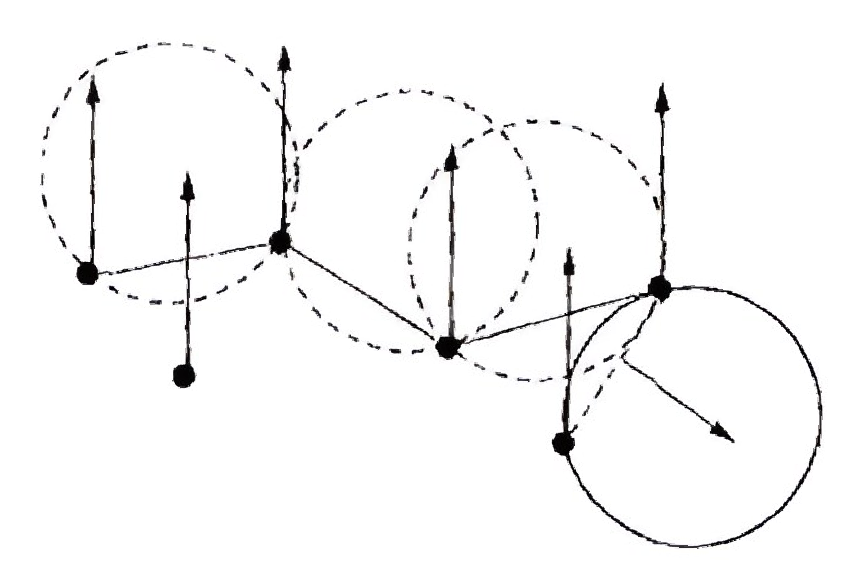
\includegraphics[scale=0.5]{2.6.eps}
\caption{三角形和顶点法线方向}
\label{fig2.6}
\end{figure}

为了提高效率，可以限制每个体素中候选点的数量，并优先考虑投影到表面法线方向的点。这种方法可以避免因噪声或不完整数据导致的小三角形组件的生成，同时减少计算资源的浪费。
\subsubsection{球旋转操作}
BPA算法中的球旋转操作是该算法的核心部分。该操作通过围绕三角形的边旋转一个球体来添加新的三角形，以逐步构建三角化表面。围绕边\( e \)进行球旋转如下图\ref{fig2.7}所示。球旋转操作的步骤分为以下几步：
\begin{figure}[htbp]
\centering
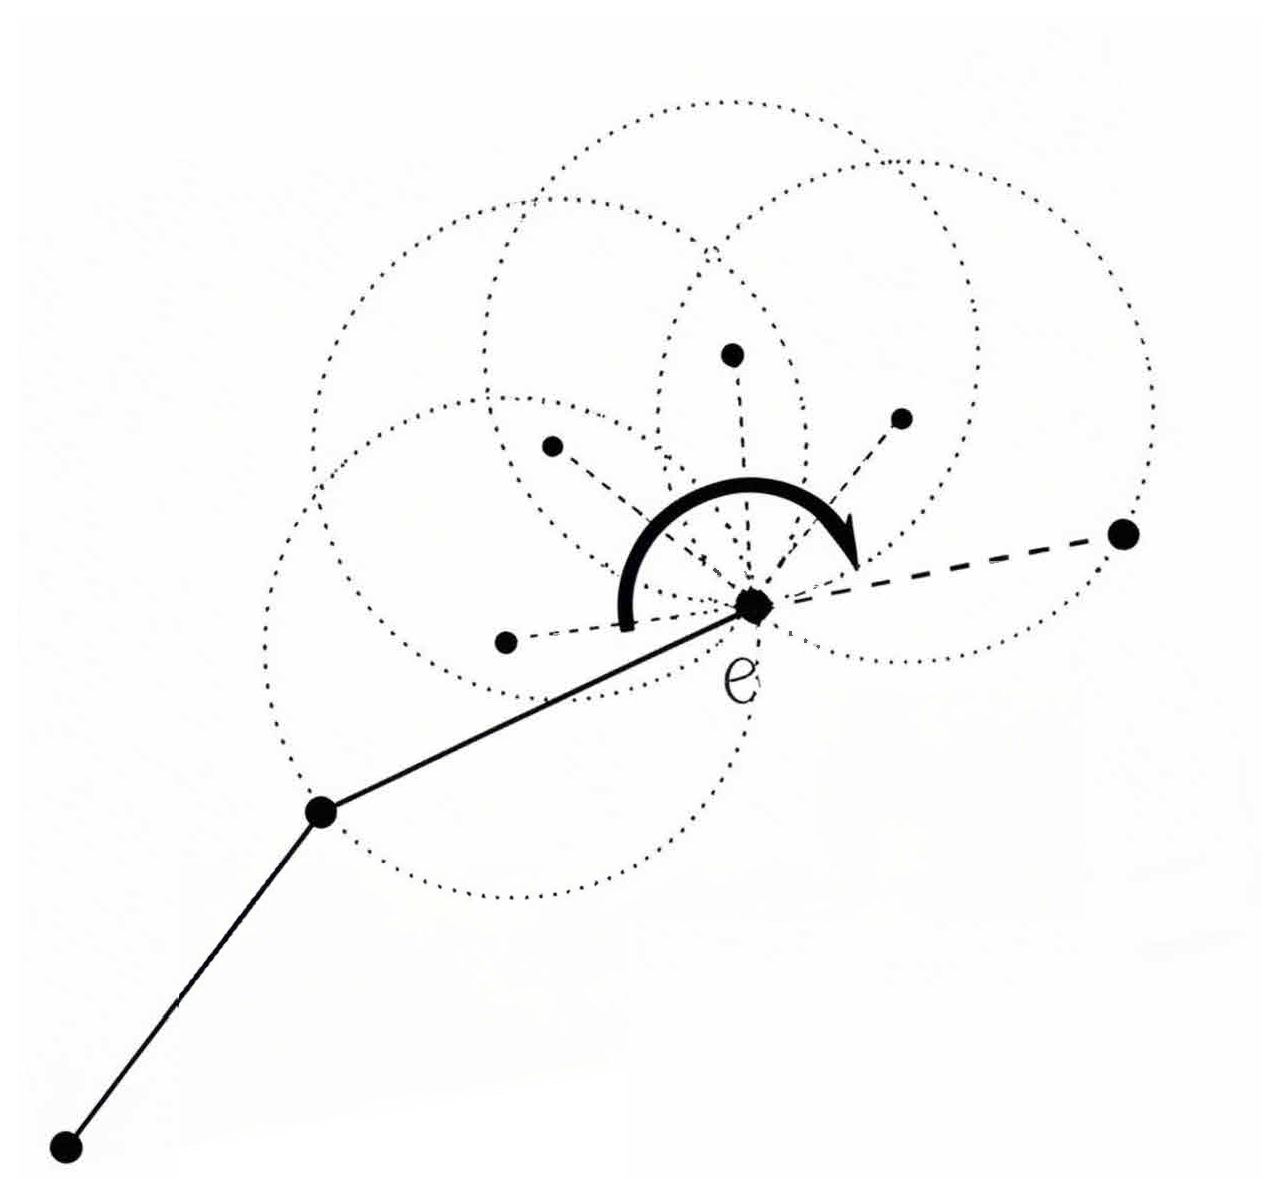
\includegraphics[scale=0.3]{2.7.eps}
\caption{旋转示意图}
\label{fig2.7}
\end{figure}

第一是初始位置，球旋转操作从一个初始三角形开始，该三角形由三个点形成，并且球体接触这三个点。球体的半径为 \( r \)，并且球体内部不包含其他数据点。

第二是旋转球体，球体围绕三角形的一条边旋转。在旋转过程中，球体保持与该边的两个端点接触，并围绕这两个点形成的轴旋转。

第三是寻找新点，在旋转过程中，球体可能会接触到另一个数据点。如果球体接触到一个新的点 \( v \)，则检查该球体是否为空（即球体内部不包含其他数据点）。

第三是创建新三角形，如果球体为空，则可以创建一个新的三角形，该三角形由旋转的边和新接触的点 \( v \) 组成。这个新三角形被添加到三角化表面中。

第四是更新前沿边，新创建的三角形的边被添加到扩展前沿边中。如果新接触的点 \( v \) 已经是其他三角形的一部分，则需要处理边的合并情况。

其中需要计算三角形外接球体的中心，对于给定的三角形 \( p, q, s \)，计算球体的中心 \( c \)，使得球体通过这三个顶点并且半径为 \( r \)。球体中心的计算步骤如下：

第一是计算三角形的外心。给定三个三维点 \( p(x_p, y_p, z_p) \)、\( q(x_q, y_q, z_q) \) 和 \( s(x_s, y_s, z_s) \)，外心 \( H(x_H, y_H, z_H) \) 是这三个点的垂直平分线的交点。外心到三个顶点的距离相等。
为了找到外心，可以构建以下方程组
\begin{align}
(x_H - x_p)^2 + (y_H - y_p)^2 + (z_H - z_p)^2 &= (x_H - x_q)^2 + (y_H - y_q)^2 + (z_H - z_q)^2 \\
(x_H - x_q)^2 + (y_H - y_q)^2 + (z_H - z_q)^2 &= (x_H - x_s)^2 + (y_H - y_s)^2 + (z_H - z_s)^2
\end{align}
通过展开和简化这些方程，可以解出外心的坐标 \( (x_H, y_H, z_H) \)。这两个方程可以写成矩阵形式
\begin{equation}
\begin{bmatrix}
x_q - x_p & y_q - y_p & z_q - z_p \\
x_s - x_q & y_s - y_q & z_s - z_q
\end{bmatrix}
\begin{bmatrix}
x_H \\
y_H \\
z_H
\end{bmatrix}
=
\begin{bmatrix}
\frac{x_q^2 + y_q^2 + z_q^2 - x_p^2 - y_p^2 - z_p^2}{2} \\
\frac{x_s^2 + y_s^2 + z_s^2 - x_q^2 - y_q^2 - z_q^2}{2}
\end{bmatrix}
\end{equation}

通过解这个线性方程组，可以得到外心的坐标 \( (x_H, y_H, z_H) \)。

其次是计算球体的中心，球体的中心 \( c \) 位于三角形平面的法线方向上，并且距离外心 \( H \) 的距离为 \( \sqrt{r^2 - r_c^2} \)，其中 \( r_c \) 是三角形的外接圆半径。球体中心的坐标可以表示为
\begin{equation}
c = H + \sqrt{r^2 - r_c^2} \cdot \frac{n}{\|n\|}
\end{equation}
其中 \( n \) 是三角形平面的法线方向。

\subsubsection{连接和粘合操作}
在BPA的扩展三角化过程中，会生成新点。此时会涉及到两种主要的操作：连接和粘合。这些操作用于处理候选顶点与当前扩展前沿边的关系，从而生成新的三角形并更新扩展前沿。

当新点未被使用时即当球绕边旋转接触到的新点尚未被网格使用时，执行连接操作。添加由该新点和边的两个端点组成的新三角形到网格中，同时从前沿边集合中移除该边，并添加新形成的两条边到前沿边集合中。

若新点已被使用：若新接触的点已属于网格中的点，首先检查添加候选新三角形是否会导致非流形顶点或非可定向流形。若不会导致这些问题，则执行连接操作，添加新三角形，并可能创建一对方向相反的重复边。

而当连接操作创建了方向相反的重复边时，执行粘合操作。移除前沿边集合中的这两条重复边，并根据情况调整前沿边的拓扑结构，确保前沿边始终是一个由链表组成的集合。

通过以上操作，BPA算法能够从点云数据中逐步构建出一个插值的三角形网格，实现对三维表面的重建。
\subsection{实现步骤}
BPA算法的操作流程可以概括成以下三个步骤。

步骤一是种子三角形选择，从尚未被重建三角网格使用的点中，考虑其邻域内的点对，构建潜在的种子三角形，并检查其有效性（如三角形法线与顶点法线方向一致，且R半径的球接触三个顶点且不包含其他数据点）。

步骤二是球旋转操作，以一个三角形的边为旋转轴，球的初始位置是接触该三角形三个顶点的位置，此时球不包含其他数据点。球保持与该边两个端点接触，沿着边的垂直平分面做圆周运动，在旋转过程中，查找球是否接触到新的数据点。这可以通过查询边两个端点邻域内的点来实现，计算这些点与当前边形成球的中心位置，判断球是否接触到其他点。若找到新点，则以该新点与边的两个端点形成新的三角形，将新三角形添加到网格中，并更新前沿边，移除旧边，添加新形成的两条边到前沿边集合中。

步骤三是连接与粘合操作，当球绕边旋转接触新点时，执行连接操作，添加新三角形并修改前沿边。若新接触的点已属于网格中的点，则根据情况执行连接或粘合操作，确保网格拓扑结构正确。

BPA算法结果示意图如下图\ref{fig2.8}所示。
\begin{figure}[htbp]
\centering
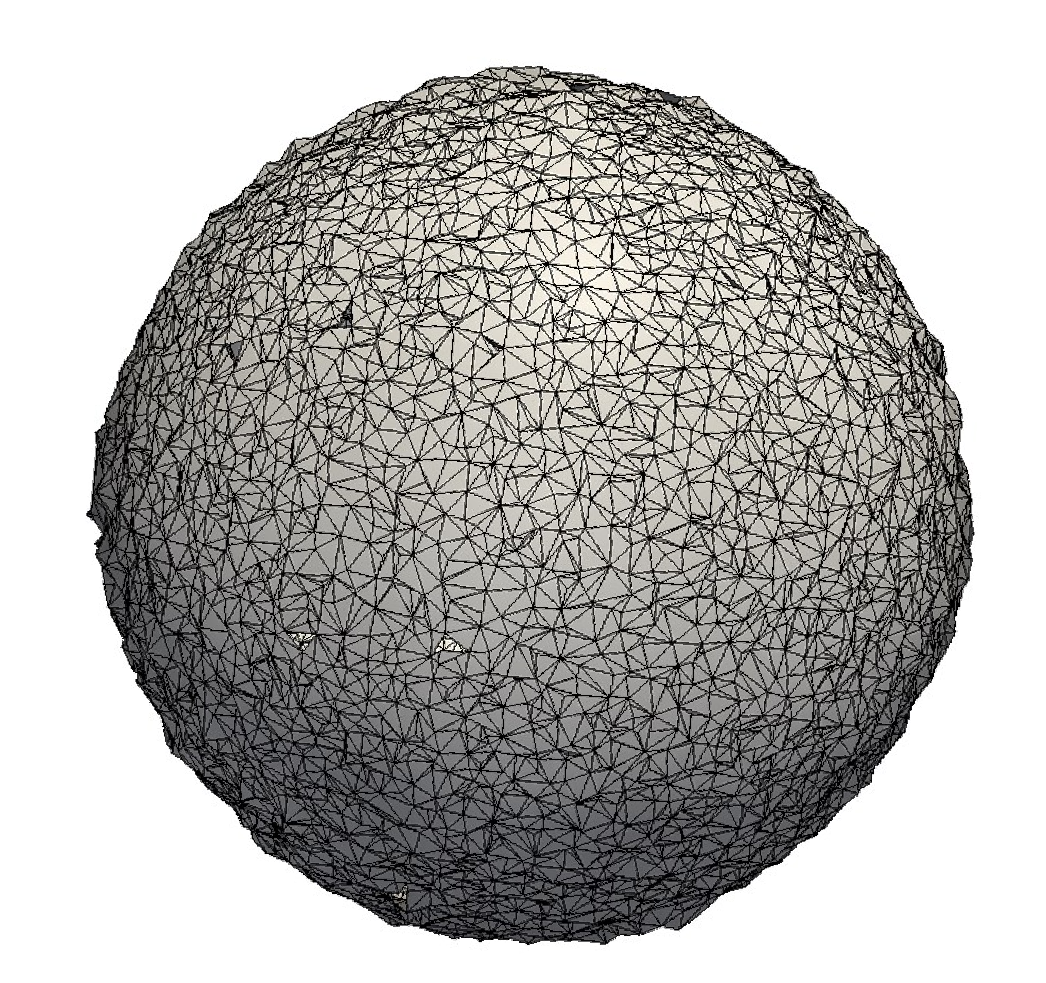
\includegraphics[scale=0.5]{2.8.eps}
\caption{ BPA结果}
\label{fig2.8}
\end{figure}
\section{本章小节}
本章详细介绍了两种传统的三维表面重建算法Alpha Shapes和BPA。Alpha Shapes算法通过参数\(\alpha\)控制形状的细节程度，基于Delaunay三角剖分实现点集的形状重建，能够捕捉从局部细节到整体结构的几何特征，但在处理非均匀采样点云和复杂形状细节时存在局限性。BPA算法通过球体旋转操作逐步构建三角化表面，适用于密集点云数据的高效表面重建，但对球体半径的选择较为敏感，半径过小会导致表面孔洞，过大则可能丢失细节。两种算法均在理论和实现层面进行了深入分析，为后续章节中隐式重建方法的研究提供了对比基础
\chapter{基于神经网络的三维表面重建研究}
\section{显式与隐式重建}
\subsection{显式重建}
三维重建是通过传感器数据（如图像、点云等）恢复场景或物体的三维几何信息的过程。根据几何信息的表示方式，三维重建可以分为显式重建和隐式重建两大类。显式重建直接构建场景的几何模型，而隐式重建通过数学函数间接描述几何形状。两者在表示方式、适用场景和处理复杂性上存在显著差异。第二章提到的两种表面重建的算法都属于显式重建的范畴。

显式重建是一种直接构建三维几何模型的方法，广泛应用于三维重建领域。其核心思想在于明确地表示场景中物体的表面或体积，以便于后续的处理和应用。显式重建的常见形式包括点云、多边形网格（尤其是三角形网格）和体素（三维像素）模型。这些形式各有特点，适用于不同的应用场景。

点云是显式重建中最基本的形式，通过一系列离散的三维点来表示场景。这些点通常包含位置信息，有时还包含颜色或法线方向等附加信息。点云数据通常来源于激光扫描或通过多视图立体重建技术从图像中提取。点云的优势在于其简单性和灵活性，可以快速获取大量数据，适用于大规模场景的初步重建。然而，点云缺乏拓扑信息，难以直接用于复杂的几何处理和渲染。

多边形网格是显式重建中另一种常见的表示形式，通过连接的多边形（通常是三角形）来表示物体的表面。多边形网格能够提供详细的表面信息，并且可以包含纹理映射，使其在计算机图形学中得到广泛应用。三角形网格因其计算稳定性和易于处理的特性，成为最常用的多边形网格形式。多边形网格不仅能够精确表示复杂的几何形状，还能通过简化或细分操作来适应不同的精度需求。然而，对于非常复杂的场景，多边形网格可能会变得非常庞大，导致存储和处理的困难。

体素是显式重建中的另一种表示方式，通过三维像素（体素）来表示场景。每个体素包含一个位置和一个值，表示该位置的属性（如密度或颜色）。体素模型特别适合处理体积数据，如医学成像或地质建模。然而，体素模型的存储开销较大，尤其是在高分辨率情况下，这限制了其在大规模场景中的应用。

显式重建的一个显著特点是其直观性。显式模型能够直接呈现几何形状，使得用户可以轻松地可视化和编辑这些模型。这种直观性使得显式重建在许多需要直接操作三维数据的应用中非常受欢迎，如建筑设计、文物保护和虚拟现实等。此外，显式模型与大多数3D处理和渲染软件高度兼容，便于后续的处理和应用。这种兼容性使得显式重建成为许多实际项目中的首选方法。

然而，显式重建也存在一些局限性。对于复杂场景，多边形网格可能变得非常庞大，导致存储和处理的困难。这种复杂性不仅增加了计算成本，还可能限制模型的可用性。此外，显式重建在处理物体的拓扑变化时可能较为困难。例如，当物体发生断裂或合并时，显式模型需要重新构建或调整，这可能涉及到复杂的算法和大量的计算资源。这些局限性使得显式重建在某些特定场景下可能不如隐式重建灵活和高效
\subsection{隐式重建}
隐式重建是一种基于隐式函数的三维重建方法，其核心思想是通过一个连续的数学函数来描述场景中每一点的几何属性。隐式函数通常定义为标量场，通过该函数的零等值面来表示物体的几何边界。这种方法与显式重建不同，它并不直接构建物体的表面或体积，而是通过隐式函数的数学形式间接描述几何形状。隐式重建的灵活性和高效性使其在复杂场景和高精度需求的应用中具有显著优势。

隐式重建的一个显著特点是其连续性。通过隐式函数的数学表达，隐式重建能够以任意精度表示复杂的表面和结构。这种连续性使得隐式模型在处理精细的几何细节时表现优异，例如在高质量的3D场景渲染和电影特效中，隐式重建能够捕捉到物体表面的微小变化，提供更加逼真的视觉效果。此外，隐式重建的灵活性体现在其对拓扑变化的自然处理能力上。与显式重建相比，隐式重建不需要显式地跟踪物体的拓扑结构，因此能够轻松应对复杂的拓扑变化，如物体的断裂、合并或变形。这种灵活性使得隐式重建在动态场景或复杂几何结构的重建中具有明显优势。

隐式重建的紧凑性也是其一大特点。通过隐式函数的数学形式，隐式重建能够使用较少的参数描述复杂的场景。这种紧凑性不仅减少了存储需求，还提高了计算效率，使得隐式模型在处理大规模场景时更加高效。例如，在符号距离场中，每个空间点的符号距离值可以精确地表示其与物体表面的相对位置，而无需显式地存储整个表面的几何信息。这种表示方式在处理复杂场景时尤为有效，因为它能够在保持高精度的同时显著降低存储和计算成本。

隐式重建的常见方法包括符号距离场、神经辐射场和占有场。符号距离场通过标量函数表示空间点与物体表面的距离，符号表示内外关系。这种方法在处理复杂几何形状时具有很高的精度，同时能够自然地处理拓扑变化。神经辐射场则通过神经网络隐式地表示场景的几何和外观信息，能够实现高质量的3D场景重建和渲染。这种方法在处理光照效果和复杂几何结构时表现尤为突出，成为近年来研究的热点。占有场通过标量函数表示空间点是否在物体内部，这种方法简单直观，适用于某些特定的应用场景。

尽管隐式重建具有许多优势，但它也存在一些局限性。首先，隐式表示的3D模型在直接编辑时较为困难。由于隐式模型是通过数学函数间接描述的，直接修改其几何形状需要复杂的计算和优化过程，这在实际应用中可能会带来一定的挑战。其次，隐式模型的渲染和处理通常需要复杂的计算。与显式模型相比，隐式模型的渲染过程需要通过隐式函数的计算来生成表面信息，这可能导致计算成本较高，尤其是在实时应用中。

隐式重建的适用场景主要集中在需要高精度3D模型或处理复杂场景和光照效果的应用中。例如，在高质量的3D场景渲染中，隐式重建能够捕捉到物体表面的精细细节，提供更加逼真的视觉效果。在电影特效中，隐式重建的灵活性和高效性使其能够轻松处理复杂的动态场景和拓扑变化。此外，在精细的3D模型重建中，隐式重建能够通过符号距离场或神经辐射场等方法实现高精度的几何和外观重建，满足对细节和精度的高要求。相比之下，显式重建更适合于需要直接操作或实时处理3D几何数据的应用，如机器人导航、实时监控和交互式虚拟现实。在这些场景中，显式模型的直观性和实时性使其成为更合适的选择。
\section{有向距离函数}
有向距离函数（Signed Distance Function，简称SDF）是一种用于表示空间中点与几何形状相对位置关系的数学函数。它通过为每个点赋予一个有符号的距离值来描述该点与几何形状边界的距离关系。

SD可以更详细地定义如下：

给定一个空间 \( \mathcal{O} \) 和该空间中的一个几何形状 \( B \)，对于空间 \( \mathcal{O} \) 中的任意一点 \( \mathbf{x} \)，SDF将该点映射到一个实数值，表示该点到几何形状 \( B \) 边界的最短距离。具体来说

\begin{equation}
SDF(\mathbf{x}) = 
\begin{cases} 
- \min_{\mathbf{y} \in \partial B} \left\| \mathbf{x} - \mathbf{y} \right\|, & \text{若 } \mathbf{x} \in \text{内部}(x), \\
+ \min_{\mathbf{y} \in \partial B} \left\| \mathbf{x} - \mathbf{y} \right\|, & \text{若 } \mathbf{x} \in \text{外部}(B), \\
0, & \text{若 } \mathbf{x} \in \partial B.
\end{cases}
\end{equation}
其中\( \mathbf{x} \) 表示空间 \( \mathcal{O} \) 中的一个点。
\( \partial B \) 表示几何形状 \( B \) 的边界。
 \( \text{内部}(B) \) 表示几何形状 \( B \) 的内部区域。
\( \text{外部}(B) \) 表示几何形状 \( B \) 的外部区域。
\( \left\| \mathbf{x} - \mathbf{y} \right\| \) 表示点 \( \mathbf{x} \) 到边界点 \( \mathbf{y} \) 的欧几里得距离。
这个定义不仅包含了距离信息，还通过符号表示了点 \( \mathbf{x} \) 相对于几何形状 \( B \) 的位置关系。

从数学的角度来看，SDF可以被视为一个标量场，它在空间中的每个点都关联一个标量值，即该点到最近边界的有符号距离。这个标量场不仅包含了距离信息，还包含了方向信息，即点是在边界内部还是外部。

此外，SDF还可以被视为Eikonal方程的一个特例，其形式为
\begin{equation}
\| \nabla SDF(\mathbf{x}) \| = 1
\end{equation}

其中，$\nabla$ 表示梯度算子。这个方程表明，SDF的梯度的模在空间中是恒定的，这使得SDF在处理几何形状时具有良好的数学性质和计算效率。

SDF在多个领域具有广泛的应用，尤其是在计算机图形学和物理模拟中。例如，在计算机图形学中，SDF可以用于生成抗锯齿的图形、进行碰撞检测以及实现复杂的几何建模。在物理模拟中，SDF可以用于描述物体的边界，从而实现精确的碰撞响应和流体模拟。此外，SDF还可以用于3D建模、程序化生成、软阴影渲染、流体模拟与交互等领域。
\section{多层感知机表示SDF}
多层感知机（MultilayerPerceptron,MLP）是一种前馈神经网络，由输入层、一个或多个隐藏层以及输出层组成。每个神经元都与前一层的所有神经元相连，不存在同层连接或跨层连接。MLP通过激活函数引入非线性，使其能够学习复杂的输入输出映射关系。多层感知机如下图\ref{fig3.1}所示。
\begin{figure}[htbp]
\centering
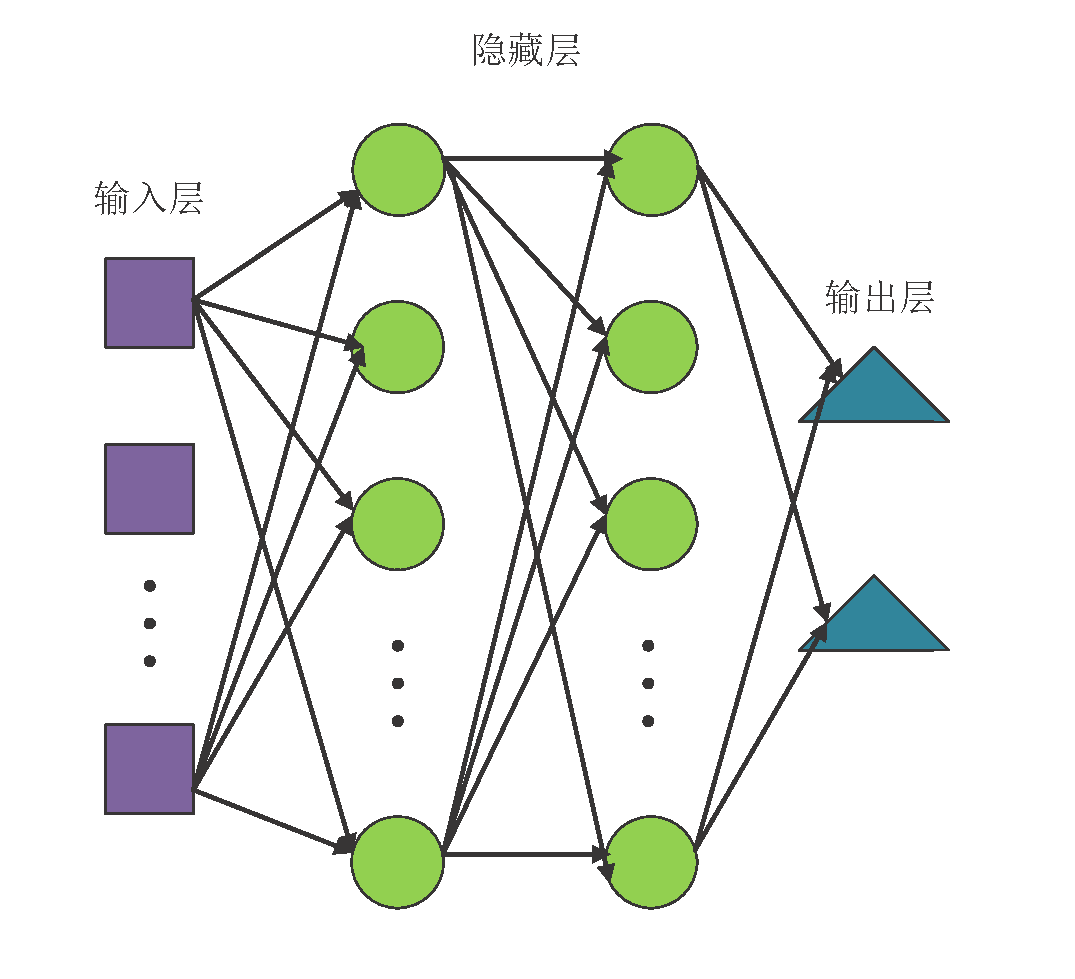
\includegraphics[scale=0.7]{3.1.eps}
\caption{多层感知机示意图}
\label{fig3.1}
\end{figure}
MLP的数学模型可以表示为，假设输入向量为\( \mathbf{x} \in \mathbb{R}^n \)，权重矩阵为\( \mathbf{W} \in \mathbb{R}^{m \times n} \)，偏置项为\( \mathbf{b} \in \mathbb{R}^m \)，激活函数为\( \sigma \)，则隐藏层的输出可以表示为：
\begin{equation}
\mathbf{h} = \sigma(\mathbf{Wx} + \mathbf{b})
\end{equation}

输出层的输出为：
\begin{equation}
\mathbf{y} = \sigma(\mathbf{W'}\mathbf{h} + \mathbf{b'})
\end{equation}
其中，\( \mathbf{W'} \in \mathbb{R}^{k \times m} \)和\( \mathbf{b'} \in \mathbb{R}^k \)分别是输出层的权重矩阵和偏置项。

激活函数\( \sigma \)是MLP中引入非线性的关键，常见的激活函数包括

\textbf{ReLU}：
\begin{equation}
\sigma(z) = \max(0, z)
\end{equation}
\textbf{Sigmoid}：
\begin{equation}
\sigma(z) = \frac{1}{1 + e^{-z}}
\end{equation}
\textbf{Tanh}：
\begin{equation}
\sigma(z) = \tanh(z)
\end{equation}

在MLP中，输入层接收输入数据，隐藏层通过非线性变换提取特征，输出层给出预测结果。隐藏层的数量和神经元数量是超参数，需要根据具体问题进行调整。激活函数的选择也会影响模型的性能，常见的激活函数包括Sigmoid、ReLU等。

MLP的工作原理包括信号的前向传播和误差的反向传播。在前向传播过程中，输入数据依次通过各层神经元，经过加权求和和激活函数变换，最终得到输出结果。在反向传播过程中，计算预测结果与真实标签之间的误差，并从输出层开始反向传播误差，计算每一层的权重和偏置的梯度，根据梯度更新权重和偏置，使得误差逐渐减小。通过不断地重复前向传播和反向传播过程，MLP逐渐调整权重和偏置，学习到输入数据和输出目标之间的映射关系，从而实现对新数据的准确预测和分类等任务。

在DeepSDF中，作者首次尝试用MLP来隐式的表示SDF，通过缩小MLP的输出和真实SDF的差来让MLP拟合一个SDF。MLP通过学习将三维坐标 \(\mathbf{x}\) 映射到SDF值，即
\begin{equation}
f_\theta(\mathbf{x}) \approx \phi(\mathbf{x}), \forall \mathbf{x} \in \Omega 
\end{equation}
其中，\( f_\theta \) 是由参数 \(\theta\) 定义的MLP。

损失函数为
\begin{equation}
\mathcal{L}(f_\theta(\mathbf{x}), \phi(\mathbf{x})) = \left| \text{clamp}(f_\theta(\mathbf{x}), \delta) - \text{clamp}(\phi(\mathbf{x}), \delta) \right| 
\end{equation}
其中，\(\text{clamp}(v, \delta)\) 是一个将值 \(v\) 限制在 \([- \delta, \delta]\) 范围内的函数，以避免梯度爆炸或消失的问题。 

MLP凭借其灵活性和强大的非线性建模能力，在三维重建领域展现出显著优势。通过结合Eikonal Loss和其他约束项，MLP能够有效稳定优化SDF的表示，并在复杂几何结构的重建中取得优异效果。

对于非表面点，MLP需要获取符号信息以及到表面的距离信息。然而，在许多实际应用中，获取真实SDF往往较为困难。为了解决这一问题，SAL提出了一种几何初始化方法，即将MLP的输出初始化为一个球形结构。这种初始化方法不仅提高了训练的稳定性，还在后续的研究中被广泛应用，成为一种重要的技术手段。
\section{StEik}
\subsection{Eikonal Loss}
在IGR中，作者提出了一种基于Eikonal Equation的限制条件，该条件能够促使所学函数逼近符号距离函数。这种限制条件在存在或不存在法线信息的情况下均能发挥作用。作者进一步证明，仅通过这种限制条件与对表面点SDF值为零的约束相结合，便足以学习到理想的SDF，而无需采用SAL中提出的复杂学习方法。这一限制条件后来发展成为著名的Eikonal Loss，成为三维重建领域中不可或缺的约束条件。

Eikonal Loss 是一种基于 Eikonal 方程的损失函数，其核心目标是促使生成的距离场满足特定的传播速度条件。Eikonal 方程的形式为
\begin{equation}
\|\nabla D(x)\|_2 = F(x),
\end{equation}
其中 \( D(x) \) 是距离场，\( F(x) \) 是传播速度。在符号距离函数的中，理想情况下，SDF 的梯度模长应为 1。简单证明为，符号距离函数 \( D(p) \) 表示点 \( p \) 到表面 \( S \) 的有符号距离。对于表面 \( S \) 上的点 \( q \)，有 \( D(q) = 0 \)。对于表面外的点 \( p \)，\( D(p) > 0 \)；对于表面内的点 \( p \)，\( D(p) < 0 \)。假设点 \( p \) 到表面 \( S \) 的距离为 \( d \)，则 \( D(p) = d \)。沿着从 \( p \) 到 \( S \) 的方向（即梯度方向），函数值的变化率应为 1，因为每移动一个单位的距离，函数值就变化一个单位。
    
数学上，这可以表示为：
\begin{equation}
\frac{dD}{ds} = 1,
\end{equation}
其中 \( s \) 是沿梯度方向的距离。

根据链式法则，梯度方向上的变化率可以表示为
\begin{equation}
\nabla D \cdot \frac{d\mathbf{p}}{ds} = 1.
\end{equation}

由于 \( \frac{d\mathbf{p}}{ds} \) 是沿梯度方向的单位向量，因此
\begin{equation}
\|\nabla D\|_2 \cdot \left\| \frac{d\mathbf{p}}{ds} \right\|_2 = 1.
\end{equation}

因为 \( \frac{d\mathbf{p}}{ds} \) 是单位向量，所以
\begin{equation}
\|\nabla D\|_2 = 1.
\end{equation}

因此 Eikonal Loss 通常定义为
\begin{equation}
L_{\text{Eik}} = \sum_{p \in R} \left( \|\nabla D(p)\|_2 - 1 \right)^2,
\end{equation}
其中 \( R \) 是一组采样点

Eikonal Loss 在表面重建中扮演着关键角色。通过约束 SDF 的梯度模长为 1，Eikonal Loss 确保生成的距离场符合符号距离函数的几何特性。具体来说,Eikonal Loss 强制 SDF 的梯度方向指向最近的表面，并确保梯度模长为 1，从而保证距离场的正确性。尽管 Eikonal Loss 在表面重建中具有重要作用，但其优化过程可能存在不稳定性，例如当网络的表达能力增强时，Eikonal Loss 的优化过程可能会变得不稳定，导致优化陷入局部最小值或生成不合理的几何结构。

为了解决这些问题，近年来的研究提出了一些改进方法，例如通过引入方向散度正则化来稳定 Eikonal Loss 的优化过程。这些方法在保持 Eikonal Loss 的核心作用的同时，显著提高了表面重建的精度和稳定性。
\subsection{StEik算法介绍}
StEik（Stabilizing the Eikonal Equation）是一种创新性的方法，旨在通过引入新的正则化约束和优化的网络架构，稳定神经符号距离函数（SDF）的优化过程，并实现对复杂形状的精细和准确表示。该方法的核心目标是解决传统神经隐式表示（INR）方法中eikonal约束优化不稳定的难题。

在传统的神经隐式表示方法中，符号距离函数通常被用于隐式地表示形状，其中形状的表面被定义为SDF的零水平集。然而，现有的方法在优化过程中常常面临一个关键问题，随着网络表示能力的增强，用于约束SDF的Eikonal Loss可能导致优化过程的不稳定性。这种不稳定性不仅会引发重建表面的异常，还可能导致优化陷入次优的局部最小值，从而无法准确捕捉形状的细微几何和拓扑结构。

StEik方法通过引入方向散度正则化项来解决这一问题。该正则化项能够有效地稳定Eikonal Loss的优化过程，从而避免了传统方法中可能出现的不稳定性。实验结果表明，StEik在多个数据集上的表现均优于现有的最先进方法，尤其是在重建薄结构方面表现出色。此外，StEik方法在参数数量上也具有优势，与DiGS方法相比，StEik在使用更少参数的情况下仍然能够取得更好的结果。这表明StEik不仅提高了重建的精度，还提高了模型的效率。

为了解决这一问题，StEik方法基于几何偏微分方程理论，对神经SDF的优化过程进行了深入的理论分析。发现当网络的表示能力逐渐增强以恢复更精细的形状特征时，优化过程在连续极限下可能变得不稳定。这种不稳定性源于Eikonal Loss的梯度下降偏微分方程，在某些情况下会导致优化过程发散或产生不期望的振荡。

基于这一理论分析，StEik提出了一种新的正则化项——法线方向的散度。这一正则化项通过约束SDF的Hessian矩阵在法线方向上的二阶导数为零，有效地稳定了Eikonal Loss的优化过程。与现有的正则化方法（如散度损失和法线约束）相比，StEik的新正则化项不仅能够稳定优化过程，还能避免过度正则化导致的形状细节丢失。这是因为传统的散度损失会惩罚SDF的Laplacian，从而对形状的平均曲率施加约束，这在某些情况下可能会导致形状的过度平滑，尤其是对于具有复杂曲率的形状。而StEik的法线方向散度正则化项则专注于稳定优化过程，同时允许形状的局部几何特征得以保留。

StEik 的总损失函数定义为：
\begin{equation}
L = \alpha_e L_{eik} + \alpha_m L_{manifold} + \alpha_n L_{nonmanifold} + \alpha_l L_{L,n}
\end{equation}
其中
 \(\alpha_e, \alpha_m, \alpha_n, \alpha_l\) 是超参数，用于平衡不同损失项的权重。
\(L_{eik}\) 是 eikonal loss，用于约束 SDF 的梯度模长为 1。
  \(L_{manifold}\) 是 manifold loss，用于惩罚远离零水平集的点。
  \(L_{nonmanifold}\) 是 non-manifold loss，用于惩罚非目标表面的点靠近零水平集。
\(L_{L,n}\) 是 directional divergence loss，用于稳定 eikonal loss 的优化过程，同时避免过度平滑。

Eikonal Loss 定义为：
\begin{equation}
L_{eik}(u) = \frac{1}{2} \int_{\Omega} \left| \left| \nabla u(x) \right| - 1 \right|^p dx
\end{equation}
其中
\(\nabla u(x)\) 是 SDF \(u(x)\) 的梯度。
\(p\) 是损失的阶数，通常取 1 或 2。当 \(p = 1\) 时，损失为绝对值形式；当 \(p = 2\) 时，损失为平方形式。
该损失项确保 SDF 的梯度模长接近 1，从而满足符号距离函数的几何特性。

Manifold Loss 定义为：
\begin{equation}
L_{manifold}(u) = \frac{1}{2} \int_{\Omega \setminus \Omega_0} \exp(-\alpha |u(x)|) dx
\end{equation}
其中
\(\Omega\) 是整个定义域。
\(\Omega_0\) 是已知表面点（例如点云数据）的集合。
\(\alpha\) 是一个正则化参数，用于控制惩罚的强度。
该损失项惩罚远离零水平集的点，确保重建的形状集中在目标表面附近。

Non-Manifold Loss 定义为：
\begin{equation}
L_{nonmanifold}(u) = \frac{1}{2} \int_{\Omega_0} |u(x)| dx
\end{equation}
其中：\(\Omega_0\) 是已知表面点的集合。
该损失项惩罚非目标表面的点靠近零水平集，避免重建出不需要的几何结构。

Directional Divergence Loss 定义为
\begin{equation}
L_{L,n}(u) = \int_{\Omega} \nabla u(x)^T D^2(x) \cdot \nabla u(x) dx
\end{equation}
其中\(\nabla u(x)\) 是 SDF \(u(x)\) 的梯度。
\(D^2(x)\) 是 Hessian 矩阵，表示 SDF 的二阶导数。该损失项约束 SDF 的二阶导数在法线方向为零，从而稳定 eikonal loss 的优化过程，同时避免过度平滑。

StEik 方法通过结合上述损失项，有效地稳定了神经 SDF 的优化过程，并允许形状的局部几何特征得以保留。

此外，StEik还引入了一种新的网络结构——基于二次层的神经网络。这种网络结构的核心思想是利用二次函数的组合来近似更高阶的多项式函数，从而实现对形状更精细的分段多项式表示。与传统的基于线性层的神经网络相比，二次层网络能够以更少的网络参数捕捉到形状的复杂几何特征，例如薄结构和尖锐边缘等。这种网络结构的引入，使得StEik能够在不牺牲优化稳定性的情况下，显著提升形状重建的质量和细节表现。

将 MLP 的线性层替换为如下表示的二次函数层，即
\begin{equation}
a(\mathbf{x}) = (\mathbf{W}_1 \mathbf{x} + b_1) \circ (\mathbf{W}_2 \mathbf{x} + b_2) + \mathbf{W}_3 \mathbf{x}^2 + b_3
\end{equation}
其中
\( \mathbf{x} \in \mathbb{R}^{m_2} \) 是输入向量。
\( \mathbf{W}_1 \in \mathbb{R}^{m_1 \times m_2} \) 和 \( \mathbf{W}_2 \in \mathbb{R}^{m_1 \times m_2} \) 是权重矩阵。
\( b_1 \in \mathbb{R}^{m_1} \) 和 \( b_2 \in \mathbb{R}^{m_1} \) 是偏置向量。
\( \mathbf{W}_3 \in \mathbb{R}^{m_1 \times m_2} \) 是二次项的权重矩阵。
\( b_3 \in \mathbb{R}^{m_1} \) 是二次项的偏置向量。
\( \circ \) 表示元素乘积。

在各种数据集上，StEik的效果相比于先进方法有较大提升，尤其是在处理复杂形状和薄结构时表现出色，此外，在大规模场景重建任务中，StEik能够恢复出更多精细的形状细节，如图片框架和沙发腿等薄结构，而现有方法往往会出现过度平滑的问题。
\section{本章小节}
第三章详细探讨了基于神经网络的三维表面重建技术，分析了显式与隐式重建方法的特点及其在三维重建中的应用。显式重建方法虽然直观且易于操作，但在处理复杂几何结构和拓扑变化时存在局限性。相比之下，隐式重建方法通过数学函数间接描述几何形状，展现出更高的灵活性和高效性，尤其在处理复杂场景和高精度需求的应用中具有显著优势。

本章深入研究了隐式重建中的有向距离函数，并探讨了如何利用多层感知机来表示SDF。通过结合Eikonal Loss和其他约束项，MLP能够有效稳定优化SDF的表示，并在复杂几何结构的重建中取得优异效果。此外，本章还介绍了StEik算法，这是一种创新性的方法，通过引入方向散度正则化项和优化的网络架构，稳定神经符号距离函数SDF的优化过程，并实现对复杂形状的精细和准确表示。

StEik算法在多个数据集上的表现优于现有的最先进方法，尤其是在重建薄结构方面表现出色。此外，StEik方法在参数数量上也具有优势，能够在使用更少参数的情况下取得更好的结果。这表明StEik不仅提高了重建的精度，还提高了模型的效率。通过结合方向散度损失和其他损失项，StEik有效地稳定了神经SDF的优化过程，并允许形状的局部几何特征得以保留。此外，基于二次层的神经网络结构的引入，使得StEik能够以更少的网络参数捕捉到形状的复杂几何特征，从而显著提升形状重建的质量和细节表现。
\chapter{三维表面重建算法的仿真验证}
\section{算法介绍}

\chapter{总结与展望}
\end{document}
